%%% XeLaTeX-article %%%
%# -*- coding: utf-8 -*-
%!TEX encoding = UTF-8 Unicode
%!TEX TS-program = xelatex
%---------------------虽然加了%还是要保留！

\documentclass[17pt]{beamer}
\mode<presentation>
{
\usetheme[width=40pt]{Hannover}
\usecolortheme[]{dove}
\usefonttheme[]{structurebold}
\setbeameroption{hide notes}
}

\usepackage{fontspec}
\usepackage{polyglossia}
\setmainfont{Arial} %设置主字体
\newfontfamily\sanskritfont[Script=Devanagari,Mapping=romantodevanagari,Scale=1.15]{Sanskrit 2003}             %输出天城体
%\newfontfamily\sanskritfont[Mapping=tex-text]{Times New Roman}              %输出转写
\doublehyphendemerits=-10000
\newcommand{\skt}[1]{{\sanskritfont{#1}}} %输出天城体
\newcommand{\skttrans}[1]{{\skt{#1}~#1}}  %输出天城体和转写
%----------------------------------------------------设置梵文输入方法 danda । ॥

\usepackage[UTF8,fontset=windows]{ctex}
\usepackage{amsmath}
%----------------------------------------------------设置中文环境

\usepackage{graphicx}
\usepackage{flafter}
\graphicspath{{pic/}}
\usepackage{booktabs}
\usepackage{nicematrix}
\newenvironment{indentlist}
  {\begin{list}{}{\setlength{\leftmargin}{2em}\setlength{\itemsep}{0.5em}}}
  {\end{list}}
%-----------------------------------------插图表格

\usepackage{hyperref}
\usepackage[dvipsnames]{xcolor}
\usepackage{colortbl}
\definecolor{light-gray}{gray}{0.9}
%------------------------------颜色

\newcommand{\verbroot}[1]{\textcolor{red}{$\sqrt{}$#1}}
\newcommand{\sktroot}[1]{{\verbroot{\skt{#1}}}}
\newcommand{\skttransroot}[1]{{\sktroot{#1}~\textcolor{red}{#1}}}

\newcommand{\nounstem}[1]{\textcolor{red}{#1\nobreakdash-}}
\newcommand{\sktnounstem}[1]{{\textcolor{red}{\skt{#1\nobreakdash-}}}}
\newcommand{\skttransnounstem}[1]{{\sktnounstem{#1}~\nounstem{#1}}}

\newcommand{\verbstem}[1]{\textcolor{blue}{#1\nobreakdash-}}
\newcommand{\sktverbstem}[1]{{\textcolor{blue}{\skt{#1\nobreakdash-}}}}
\newcommand{\skttransverbstem}[1]{{\sktverbstem{#1}~\verbstem{#1}}}

\newcommand{\wordending}[1]{\textcolor{Orange}{\nobreakdash-#1}}
\newcommand{\sktending}[1]{{\textcolor{Orange}{\skt{-#1}}}}
\newcommand{\skttransending}[1]{{\sktending{#1}~\wordending{#1}}}

\newcommand{\fullpada}[1]{\textcolor{OliveGreen}{#1}}
\newcommand{\sktpada}[1]{{\textcolor{OliveGreen}{\skt{#1}}}}
\newcommand{\skttranspada}[1]{{\sktpada{#1}~\fullpada{#1}}}

\newcommand{\pratyaya}[1]{\mbox{\textcolor{Plum}{#1}}}
\newcommand{\sktpratyaya}[1]{{\textcolor{Plum}{\skt{#1}}}}
\newcommand{\skttranspratyaya}[1]{{\sktpratyaya{#1}~\pratyaya{#1}}}

\newcommand{\reconstruction}[1]{\textcolor{gray}{*#1}}
\newcommand{\fullsentence}[1]{\textcolor{MidnightBlue}{#1}}
\newcommand{\sktsentence}[1]{\textcolor{MidnightBlue}{\skt{#1}}}

\newcommand{\veryimportant}[1]{\textcolor{red}{#1}}
\newcommand{\important}[1]{\textcolor{blue}{#1}}
\newcommand{\notsoimportant}[1]{\textcolor{gray}{#1}}
\newcommand{\dicturl}[2]{\href{#1}{\mbox{\texttt{#2}}}}
%-------------------------------------------词根等标颜色

\title{{梵语提高}}
\subtitle{34. 迂回完成时；\\以 -na结尾的过去分词}
\author[张雪杉]{文学院~~张雪杉 \\ zhangxueshan@sdnu.edu.cn}
\date{}

\begin{document}

\begin{frame}
  \titlepage
\end{frame}

\begin{frame}
  \frametitle{本节内容}
  \small
  \tableofcontents
\end{frame}

\section{上节作业}

\begin{frame}{第33章练习1}
  \small
  \begin{verse}
    \skt{1) vacanāni śrotavyāni śuśrūṣāmaḥ ।}\\
    \mbox{\skt{2) ādau na ko 'pi cāpena saśareṇāyuyutsata ।}}\\
    \skt{3) apīha nadītīrasya samīpe tatra vā vṛkṣasya chāyāyāṃ suṣupsasi ।}\\
    \skt{4) pure jigamiṣāmi rājānaṃ ca didṛkṣāmi ।}\\
    \skt{5) satyaṃ sarvairvacanīyaṃ śravaṇīyaṃ ca ।}\\
    \mbox{\skt{6) yasyāḥ kanyāyāstadratnamapāharastasyai pratideyam ।}}\\
    \skt{7) te sarve yatnaṃ cikīrṣavo 'pyatra tiṣṭhanti na ca kaścitkiṃ cana karoti ।}\\
  \end{verse}
\end{frame}



\begin{frame}{第33章练习1}
  \small
  \begin{verse}
    \skt{8) arīnāśubhiḥ \veryimportant{śarairjighāṃsati} ।}\\
    \skt{9) kanyāyā īpsā mahatyā rājñyā rucirāṇi ratnāni draṣṭuṃ spraṣṭuṃ cāsīt । kanyā rājñyā rucirāṇi ratnānyadidṛkṣadapispṛkṣacca ।}\\
    \skt{10) anayordevyoḥ katarā pūjanīyatareti naraḥ kaviṃ pipṛcchiṣati ।}\\
    \skt{11) bālo ramaṇīye jale siṣnāsurnadyāstīraṃ dudrāva ।}\\
    \mbox{\skt{12) ahaṃ jale bahvahau snātuṃ necchāmīti kanyovāca ।}}\\
  \end{verse}
\end{frame}

\begin{frame}{第31章阅读}
  \footnotesize{
    \begin{verse}  
      \skt{dhṛtarāṣṭra uvāca}\\
      \mbox{\skt{dharmakṣetre kurukṣetre samavetā yuyutsavaḥ ।}}\\
      \mbox{\skt{māmakāḥ pāṇḍavāścaiva kimakurvata saṃjaya ।। 1-1 ।।}}\\
      \skt{saṃjaya uvāca}\\
      \skt{dṛṣṭvā tu pāṇḍavānīkaṃ vyūḍhaṃ duryodhanastadā ।}\\
      \mbox{\skt{ācāryamupasaṃgamya rājā vacanamabravīt ।। 1-2 ।।}}\\
      \skt{paśyaitāṃ pāṇḍuputrāṇāmācārya mahatīṃ camūm ।}\\
      \mbox{\skt{vyūḍhāṃ drupadaputreṇa tava śiṣyeṇa dhīmatā ।। 1-3 ।।}}\\
      \skt{atra śūrā maheṣvāsā bhīmārjunasamā yudhi ।}\\
      \mbox{\skt{yuyudhāno virāṭaśca drupadaśca mahārathaḥ ।। 1-4 ।।}}\\
    \end{verse}
  }
\end{frame}

\begin{frame}{中文翻译}
    \centering    
    
\includegraphics[width=1.0\textwidth]{bhagavatgita1.1.png}
    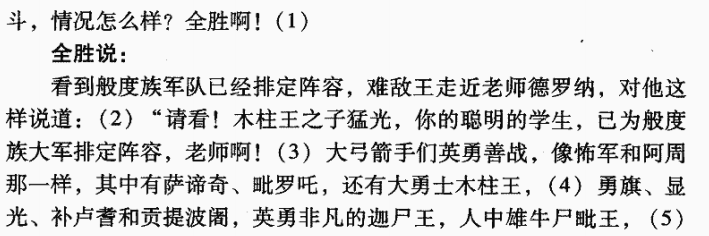
\includegraphics[width=1.0\textwidth]{bhagavatgita1.2.png}
\end{frame}

\section[迂回完成]{迂回完成时}
\begin{frame}{\insertsection}
  \small
  \tableofcontents[currentsection]
\end{frame}

\subsection{范围}
\begin{frame}{\insertsection ~~\insertsubsection}
  \begin{itemize}
    \item 两类动词使用迂回完成时代替普通完成时：
    \begin{enumerate}
      \item 派生动词：致使动词、第十类动词、愿望动词
      \item 某些以长元音开头的动词
    \end{enumerate}
  \end{itemize}
\end{frame}

\subsection{形式}
\begin{frame}{\insertsection ~~\insertsubsection}
  \small
  \begin{itemize}
    \item 现在时语干 + \pratyaya{-ām}
    \item 主动语态：加 \verbroot{as}（常用）\\
      或 \verbroot{bhū}、\verbroot{kṛ} 的完成时主动语态
    \item 中间语态：加 \verbroot{kṛ} 的完成时中间语态
  \end{itemize}
  \vspace{0.5em}
  \centering 例：\verbroot{bhṛ} \verbstem{bhāraya} → \fullpada{bhārayāmāsa} 
\end{frame}

\begin{frame}{例词}
  \small
  \centering
  \resizebox{\textwidth}{!}{
    \begin{tabular}{@{}llll@{}}
      词根 & 迂回完成时 & 人称 & 含义 \\
      \midrule
      \verbroot{bhṛ} (caus.) & \fullpada{bhārayāmāsa} & 单1 & 'caused to carry' \\
      \verbroot{bhṛ} (caus.) & \fullpada{bhārayāmāsima} & 复1 & 'we caused to carry' \\
      \verbroot{īkṣ} & \fullpada{īkṣāmāsatuḥ} & 双3 & 'the two saw' \\
      \verbroot{ās} & \fullpada{āsāṃ cakāra} & P. 单3 & 'he sat' \\
      \verbroot{ās} & \fullpada{āsāṃ cakre} & Ā. 单3 & 'he sat' \\
      \verbroot{ās} & \fullpada{āsāṃ cakrire} & Ā. 复3 & 'they sat' \\
    \end{tabular}
  }
  \vspace{0.5em}
  \begin{itemize}
    \item \notsoimportant{前三例助动词 \verbroot{as}，后三例助动词 \verbroot{kṛ}}
  \end{itemize}
\end{frame}

\begin{frame}{为何使用}
  \small
  \begin{itemize}
    \item \textbf{派生动词：}基础 \fullpada{bharati} 与致使 \fullpada{bhārayati}\\
      完成时都是 \fullpada{babhāra}，无法区分\\
      → 致使用迂回完成时：\fullpada{bhārayāmāsa}
    \item \textbf{以长元音起首的动词：}\\
      \verbroot{īkṣ} 'to see'，重复后 i + īkṣ → \fullpada{īkṣ-}\\
      与词根相同，无法识别为完成时\\
      → 用迂回完成时：\fullpada{īkṣāmāsa}
  \end{itemize}
\end{frame}




\section[na分词]{以 -na结尾的过去分词}
\begin{frame}{\insertsection}
  \small
  \tableofcontents[currentsection]
\end{frame}

\subsection{范围}
\begin{frame}{\insertsubsection}
  \begin{itemize}
    \item 大多数动词过去分词加 \pratyaya{-ta}
    \item 少数动词加 \pratyaya{-na}，含义完全相同
    \item \pratyaya{-ta} 前有时出现的联系元音 \pratyaya{-i-}\\
      不会出现在 \pratyaya{-na} 前
    \item 无法预测哪些动词用 \pratyaya{-na}
  \end{itemize}
\end{frame}

\subsection{形态}
\begin{frame}{\insertsubsection}
  \small
  \begin{itemize}
    \item 词根末 d：（词内连声 \mbox{*-d-na → -nna}）\\
      \verbroot{sad} 'to sit' → \nounstem{sanna} 'seated'
    \item 词根末 ṛ：（ṛ → īr/ūr，n → ṇ）\\
      \verbroot{stṛ} 'to strew' → \nounstem{stīrṇa} 'strewn'\\
      \verbroot{tṛ} 'to cross' → \nounstem{tīrṇa} 'crossed'
    \item 词根末元音 ā, i, u（较少）：\\
      \verbroot{kṣi} 'to destroy' \\ → \nounstem{kṣīṇa- / kṣīta} 'destroyed'  \\
    \item 常见例子：\mbox{\nounstem{vistīrṇa}} 'spread out, great'
  \end{itemize}
\end{frame}

\section{本节作业}

\begin{frame}{\insertsection }
  \begin{itemize}
    \item
      第34章练习3
    \item 第32章阅读练习？
  \end{itemize}
\end{frame}

\end{document}
